% !TEX root = Document.tex
%%
%%  Annexes.
%%
%%  Note: Ne pas modifier la ligne ci-dessous.
\addcontentsline{toc}{compteur}{ANNEXES}
\Annexe{Machine à états pour l'inspection d'éoliennes}
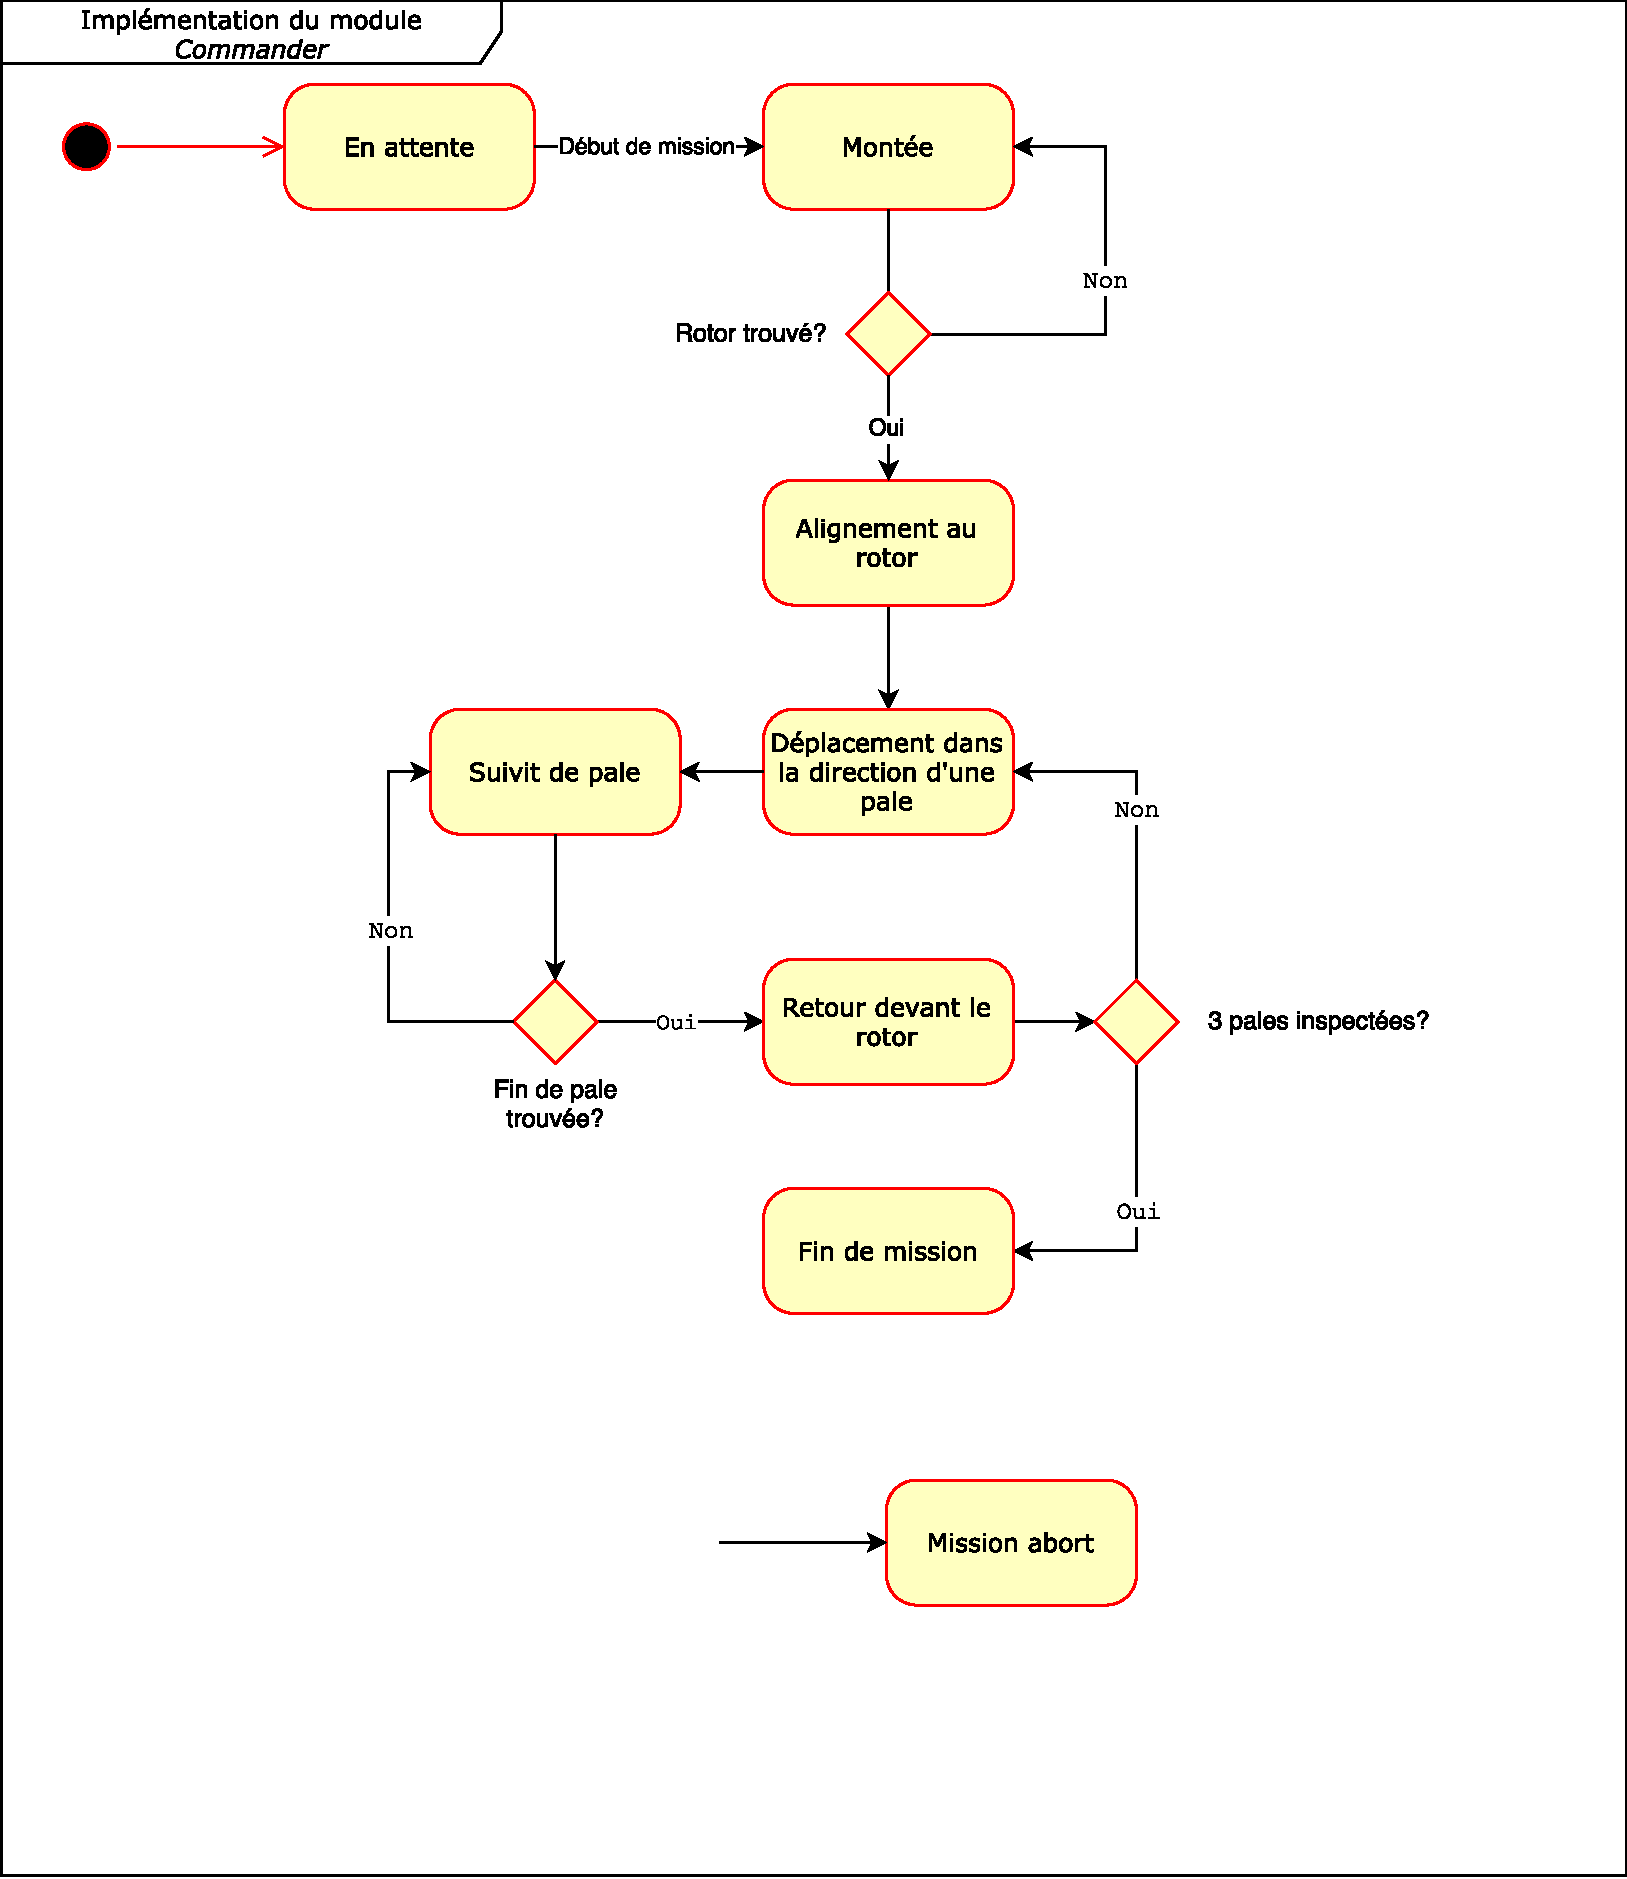
\includegraphics[width=\linewidth]{images/state_machine.pdf}
\label{annexe:state_machine}

%%
%%
%%  Toutes les annexes doivent être inclues dans ce document
%%  les unes à la suite des autres.
% \Annexe{DÉMO}
% Texte de l'annexe A\@. Remarquez que la phrase précédente se termine
% par une lettre majuscule suivie d'un point. On indique explicitement
% cette situation à \LaTeX{} afin que ce dernier ajuste correctement
% l'espacement entre le point final de la phrase et le début de la
% phrase suivante.


%\begin{landscape}
%\Annexe{ENCORE UNE ANNEXE}
%Texte de l'annexe B\@ en mode «landscape».
%\end{landscape}
%
%\Annexe{UNE DERNIÈRE ANNEXE}
%Texte de l'annexe C\@.
